\documentclass[11pt]{article}

\usepackage{graphicx}			% Use this package to include images
\usepackage{amsmath}			% A library of many standard math expressions
\usepackage{amsfonts}
\usepackage[margin=1in]{geometry}% Sets 1in margins.
\usepackage{fancyhdr}			% Creates headers and footers
\usepackage{enumerate}          %These two package give custom labels to a list
\usepackage[shortlabels]{enumitem}
\usepackage{braket}
\usepackage{physics}
\usepackage{pgfplots}
\usepackage{tikz}
\usepackage{xcolor}

\pgfplotsset{compat=1.18}

% Creates the header and footer. You can adjust the look and feel of these here.
\pagestyle{fancy}
\fancyhead[l]{Chase A. Lotito}
\fancyhead[c]{MATH450 Homework \#2}
\fancyhead[r]{\today}
\fancyfoot[c]{\thepage}
\renewcommand{\headrulewidth}{0.2pt} %Creates a horizontal line underneath the header
\setlength{\headheight}{15pt} %Sets enough space for the header



\begin{document} %The writing for your homework should all come after this.

%Enumerate starts a list of problems so you can put each homework problem after each item.
\begin{enumerate}[start=1,label={\bfseries Exercise \arabic*:},leftmargin=1in] %You can change "Problem" to be whatevber label you like.

    \item Consider a 2-dimensional manifold \(M\) with coordinate chart \(\set{x,y}\). The following objects are given:

        \begin{itemize}
            \item \(\vb{v} = 2\partial_x + \partial_y\); at point \(p = (3,1)\); \(\vb{v} \in T_p M\)
            \item \(f = x^2 + xy + 2\); scalar function; \(f \in \mathcal{F}M\)
            \item \(\vb{A} = 2x^2\partial_x + xy\partial_y\); vector field; \(\vb{A} \in \mathcal{X}M\)
            \item \(\vb{B} = y\partial_x\); vector field; \(\vb{B} \in \mathcal{X}M\)
            \item \(c(t) = (t^2 + t, 2\cos{t})\); a curve; \(\vb{c} \in \mathcal{C}M\)
        \end{itemize}

        \noindent Calculate the following:
        \begin{enumerate}
            \item \(\vb{v}f\)
            \item \(\vb{A}f\)
            \item \( f \circ c  \)
            \item \( \dv{t}(f \circ c) \) at \(t=0\)
            \item \( \dot{\vb{c}} \equiv \dot{c}(0) \)
            \item \( \dot{\vb{c}} f \)
            \item \( [\vb{A}, \vb{B}]  \)
            \item Draw the vector field \(\vb{B}\) in the neighborhood of \((0,0)\)
        \end{enumerate}

        \textbf{Solution.}

        \noindent (a)

        \begin{align*}
            \vb{v}f &= (2\partial_x + \partial_y)(x^2 + xy + 2) \\
                    &= 2 \partial_x(x^2 + xy + 2) + \partial_y(x^2 + xy + 2) \\
                    &= (2(2x + y) + x) \eval_{(x,y)=(3,1)} \\
                    &= 2(2(3)+1) + 3 \\
                    &= 17
        \end{align*}

        \noindent (b)

        \begin{align*}
            \vb{A}f &= (2x^2\partial_x + xy\partial_y)(x^2 + xy + 2) \\
                    &= 2x^2 \partial_x(x^2 + xy + 2) + xy \partial_y (x^2 + xy + 2) \\
                    &= 2x^2(2x+y) + xy(x) \\
                    &= 4x^3 + 3x^2y
        \end{align*}

        \noindent (c)

        \begin{align*}
            f \circ c &= f(c(t)) \\
                      &= (t^2 + t)^2 + (t^2 + t)(2\cos{t}) + 2
        \end{align*}

        \noindent (d)

        \begin{align*}
            \dv{t} \eval_{t=0} (f \circ c) &= \dv{t} \eval_{t=0} [(t^2 + t)^2 + (t^2 + t)(2\cos{t}) + 2 ] \\
                                                 &= 2(t^2 + t)(2t+1) + 2(2t+1)\cos{t} - \sin{t}(t^2 + t) \eval_{t=0} \\
                                                 &= 2(0)(1) + 2(1)(1) - 0(0) \\
                                                 &= 2
        \end{align*}

        \noindent (e) \emph{Remember} \(\dot{\vb{c}} = \dot{c}^i \partial_i = \dot{c}^i(x^i)\partial_i = \dv{(x^i \circ c)(t)}{t} \partial_i\). Operating on a function \(f\), \[\dot{\vb{c}}(f) = \dv{t}\eval_{t_0} f \circ c(t)\]

        \noindent Here,


        \begin{align*}
              \dot{\vb{c}} &= \dv{(t^2+t)}{t} \partial_x + \dv{(2\cos{t})}{t} \partial_y \\
                           &= (2t+1)\partial_x - (2\sin{t})\partial_y \eval_{t=0} \\
                           &= \partial_x
        \end{align*}


        \noindent (f)

        \noindent From (c), we know that \[(f\circ c) (t) = (t^2+t)^2 + (t^2+t)(2\cos{t}) + 2 \]

        So,

        \begin{align*}
            \dot{\vb{c}} f &= \dv{t} \eval_{t=t_0} (t^2+t)^2 + (t^2+t)(2\cos{t}) + 2  \\
                           &= 2(t^2+t)(2t+1) + (2t+1)(2\cos{t}) - (t^2+t)(2\sin{t}) \eval_{t=t_0} \\
                           &= 2(t_0^2+t_0)(2t_0+1) + (2t_0+1)(2\cos{t_0}) - (t_0^2+t_0)(2\sin{t_0})
        \end{align*}

        \noindent (g) \emph{Remember} the Lie bracket of two vector fields \(\vb{A}\) and \(\vb{B}\) is \[ [\vb{A}, \vb{B}] = \left( A^j(\partial_j B^i) - B^j(\partial_j A^i) \right) \partial_i\]

        \noindent Plugging in our vector fields,

        \begin{align*}
            [\vb{A}, \vb{B}] &= [ A^j ( \partial_j y ) - B^j ( \partial_j 2x^2 ) ]\partial_x + [ A^j ( \partial_j 0 ) - B^j ( \partial_j xy )  ]\partial_y \\
                             &= [ A^j ( \partial_j y ) ]\partial_x - [ B^j ( \partial_j 2x^2 ) ]\partial_x - [ B^j ( \partial_j xy )  ]\partial_y \\
                             &= [ 2x^2(\partial_x y ) + xy(\partial_y y ) ]\partial_x - [ y(\partial_x 2x^2)]\partial_x - [ y (\partial_x xy)  ]\partial_y \\
                             &= (0+xy)\partial_x - 4xy\partial_x - y^2\partial_y \\
                             &= -3xy\partial_x - y^2\partial_y \\
        \end{align*}

        \noindent (h)

        \noindent In the neighborhood of \((0,0)\),

        % Code for the vector field of B = y d_x
        \begin{center}
        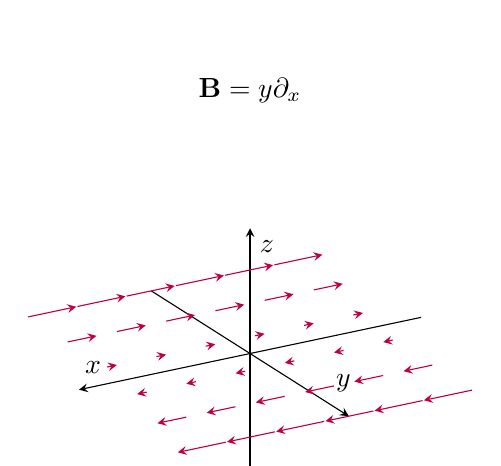
\begin{tikzpicture}
             \begin{axis}
                [
                    title = {\(\vb{B} = y \partial_x\)},
                    view={150}{30},
                    domain   = -2:2,
                    y domain = -2:2,
                    xtick    = {-2,...,2},
                    ytick    = {-2,...,2},
                    zmin=-1, zmax=1,
                    xlabel=\(x\),
                    ylabel=\(y\),
                    zlabel=\(z\),
                    ylabel style={rotate=0},
                    zlabel style={rotate=-90},
                    grid=major,
                    axis lines=middle,
                    ticks=none,
                    colormap/cool
                ]
            \addplot3[color=purple, -stealth, quiver={u=y, v=0, w=0,scale arrows=0.39}, samples=6] {0};
            \end{axis}
        \end{tikzpicture}
        \end{center}

    \item Consider \(M = \mathbb{R}^3\) with the chart of rectangular coordinates \((x,y,z)\). Express each vector of the basis associated with the chart of spherical coordinates \((r, \varphi, \theta)\), namely \(\set{\partial_r, \partial_{\varphi}, \partial_{\theta}}\) in terms of the standard basis \(\set{\partial_z, \partial_y, \partial_z}\).

        \textbf{Solution.}

    \item Show that the Lie bracket of vector fields satisfies the Jacobi identity: \[ [A, [B, C]] + [B, [C, A]] + [C, [A, B]] = 0  \]

        \textbf{Solution.}

    \item Let \(C = [A, B]\) be the Lie bracket of two vector fields. In a chart, the vector fields are given as \(A = A^i \partial_i\), \(B = B^i \partial_i\) and \(C = C^i \partial_i\). Express the coefficients \(C^i\) in terms of the coefficients of the other two vector fields.

        \textbf{Solution.}


\end{enumerate}

\end{document}
